\documentclass{book}

\title{Title}
\newcommand{\subtitle}{Subtitle}
\newcommand{\booklicense}{\href{https://creativecommons.org/licenses/by/4.0/}{Attribution
4.0 International (CC BY 4.0)}}

% authors %
\author{Stanley J. Swizzle, Jr. \and Karim F. Njdamib}
\newcommand{\authoraffiliation}{}

% Create convenient commands \booktitle and \bookauthor
\makeatletter
\newcommand{\booktitle}{\@title}
\newcommand{\bookauthor}{\@author}
\makeatother

% This utf8 declaration is not needed for versions of latex > 2018 but may
% be helpful for older software. Eventually it may not be worth keeping.
%\usepackage[utf8]{inputenc}  

\usepackage{amsmath} % Used by equations
\usepackage{hyperref}
% link options
\hypersetup{
  colorlinks=true,
  linkcolor=purple,
  urlcolor=purple,
  pdftitle={Title}
}
\usepackage{booktabs}
\usepackage{longtable}
\usepackage{array}
\usepackage{graphicx}
% sets image width to text body width
\setkeys{Gin}{width=\linewidth} 
\usepackage{xcolor}
\definecolor{purple}{HTML}{663399}

% The following dimensions specify 4.75" X 7.5" content on 6 3/8" by 9 1/4"
% paper. The paper width and height can be tweaked as required and the content
% should size to fit within the margins accordingly.
%
% The (inside) bindingoffset should be larger for books with more pages. Some
% standard recommended sizes are .375in minimum up to 1in for 600+ page books.
% Sizes .75in and .875in are also recommended roughly at 150 and 400 pages.
\usepackage[bindingoffset=1in,
            left=1in, 
            right=1in,
            top=1in, 
            bottom=1in,
            paperwidth=8.27in, 
            paperheight=11.69in]{geometry}
% Here is an alternative geometry for reading on letter size paper:
% \usepackage[margin=.75in, paperwidth=8.5in, paperheight=11in]{geometry}

\renewcommand{\contentsname}{Contents} 

% pandoc settings %
\providecommand{\tightlist}{%
  \setlength{\itemsep}{0pt}\setlength{\parskip}{0pt}}

\newenvironment{Shaded}{
    \begin{center}
    \begin{tabular}{|p{0.9\textwidth}|}
    \hline\\
    }
    { 
    \\\\\hline
    \end{tabular} 
    \end{center}
}

\newlength{\cslhangindent}
\setlength{\cslhangindent}{1.5em}
\newlength{\csllabelwidth}
\setlength{\csllabelwidth}{3em}
\newlength{\cslentryspacingunit} % times entry-spacing
\setlength{\cslentryspacingunit}{\parskip}
\newenvironment{CSLReferences}[2] % #1 hanging-ident, #2 entry spacing
 {% don't indent paragraphs
  \setlength{\parindent}{0pt}
  % turn on hanging indent if param 1 is 1
  \ifodd #1
  \let\oldpar\par
  \def\par{\hangindent=\cslhangindent\oldpar}
  \fi
  % set entry spacing
  \setlength{\parskip}{#2\cslentryspacingunit}
 }%
 {}
\usepackage{calc}
\newcommand{\CSLBlock}[1]{#1\hfill\break}
\newcommand{\CSLLeftMargin}[1]{\parbox[t]{\csllabelwidth}{#1}}
\newcommand{\CSLRightInline}[1]{\parbox[t]{\linewidth - \csllabelwidth}{#1}\break}
\newcommand{\CSLIndent}[1]{\hspace{\cslhangindent}#1}


% Content Starts Here
\begin{document}
\frontmatter

% ---- Half Title Page ----
% current geometry will be restored after title page
\newgeometry{top=1.75in,bottom=.5in}
\begin{titlepage}
\begin{flushleft}

% Title
\textbf{\fontsize{48}{54}\selectfont Title \\}
\textbf{\large \textit{Subtitle}}

% Draw a line 4pt high
\par\noindent\rule{\textwidth}{4pt}\\

% authors
\begin{flushright}

      \textbf{Stanley J. Swizzle, Jr.}, \emph{Exceptional University}\\
      \textbf{Karim F. Njdamib}, \emph{College of the Mountains}\\
  
\end{flushright}

% \vspace{\fill}
\vspace{\fill}

\end{flushleft}

\begin{center}
  %\includegraphics{booksvg.pdf}\\[4pt]
  \fontfamily{lmtt}\small{Boston Books\\
  Boston, Massachusettes\\
  https://example.com}
\end{center}
  
\end{titlepage}
\restoregeometry
% ---- End of Half Title Page ----

% Do not show page numbers on colophon page
\thispagestyle{empty}

\begin{flushleft}

\textbf{Copyright \textcopyright{} 2021  The Authors\\
License: \booklicense}\\[11pt] 

\textbf{Exceptions} \\

Except where otherwise noted, this book is licensed under a Attribution 4.0
International (CC BY
4.0). To view a copy of this license, visit https://creativecommons.org/licenses/by/4.0/

The following material is excluded from the license: 

\begin{itemize}
    \item Chapter written under a different license
    \item Image used with permission of the creator
  \end{itemize}

Chapter written under a different licenseImage used with permission of the
creator

For permissions beyond the scope of this license, visit https://example.com

\vspace*{\fill}

\begin{description}
  \item[Recommended Citation] \hfill \\ {[}Hammil, Ted. Introduction to
Statistics. Boston: Boston Books, 2021. Adapted from Jim Harris's
``Introduction to Statistics'' retrieved from
https://open.umn.edu/opentextbooks. See version notes for complete
information.{]}
  \item[Publisher] \hfill \\ Boston Books, Boston, Massachusettes
  \item[Date] \hfill \\ 2021
    \item[Website] \hfill \\ http://www.github.com
      \item[ISBN] \hfill \\ 978-0-00-867530-9 pbk.
      \item[eISBN] \hfill \\ 978-0-01-867530-9
      \item[DOI] \hfill \\ \href{https://doi.org/10.1000/xyz123}{10.1000/xyz123}
    \item[Subjects] \hfill \\ numbers game, introductory
statistics, Statistics for Undergrads
  \item[keywords] \hfill \\ statistical methods, probability, Probability, Is
there any spell-check
    \item[Contributors] \hfill \\ Elmer Bonzo, Francine Delagado
  
\end{description}

\textbf{Disclaimer} \\
  This textbook is not intended to diagonose any medical or other conditions.
  La la la

\vspace*{\fill}

This book was typeset using \LaTeX{} software and processed with \href{https://pandoc.org}{Pandoc} using the \href{http://lantern.northwestern.pub}{Lantern} publishing workflow.\\

\end{flushleft}

% A title page resets the page # to 1, but the second title page
% was actually page 3. So add two to page counter.
\addtocounter{page}{2}

% The asterisk excludes chapter from the table of contents.
\chapter*{About this Book}
This description is indentedby three spaces. Must it be? What happens if I
delete one or more of the spaces? I see also that the ``any text or symbols
go'' here \textless{} \textgreater{} \textless{} @ Just checking! chitecto
beatae vitae dicta sunt explicabo. Nemo enim ipsam voluptatem quia voluptas
sit aspernatur aut odit aut fugit, sed quia consequuntur magni dolores eos qui
ratione voluptatem sequi nesciunt. Neque porro quisquam est, qui dolorem ipsum
quia dolor sit amet, consectetur, adipisci velit, sed quia non numquam eius
modi tempora incidunt ut labore et dolore magnam aliquam quaerat voluptatem.
Ut enim ad minima veniam, quis nostrum exercitationem ullam corporis suscipit
laboriosam, nisi ut aliquid ex ea commodi consequatur? Quis autem vel eum iure
reprehenderit qui in ea voluptate velit esse quam nihil molestiae consequatur,
vel illum qui dolorem eum fugiat quo voluptas nulla pariatur?

% Three-level Table of Contents
\setcounter{tocdepth}{3}
\tableofcontents

\mainmatter

\textbf{Preface}

This work is in the public domain. Therefore, it can be copied and reproduced
without limitation.

This first chapter begins by discussing what statistics are and why the study
of statistics is important. Subsequent sections cover a variety of topics all
basic to the study of statistics. One theme common to all of these sections is
that they cover concepts and ideas important for other chapters in the book.

\hypertarget{introduction-to-vegetable-lasagna}{%
\chapter{Introduction to Vegetable
Lasagna}\label{introduction-to-vegetable-lasagna}}

\begin{itemize}
\tightlist
\item
  \textbf{First Author}, \emph{Affiliation}
\item
  \textbf{Second Author}, \emph{Affiliation}
\end{itemize}

\begin{center}\rule{0.5\linewidth}{0.5pt}\end{center}

\textbf{Learning Objectives}

\begin{itemize}
\tightlist
\item
  Objective
\item
  Objective
\item
  Objective
\end{itemize}

\begin{center}\rule{0.5\linewidth}{0.5pt}\end{center}

\hypertarget{introduction}{%
\section{Introduction}\label{introduction}}

Soup cranberry spritzer edamame hummus figs tomato and basil Bolivian rainbow
pepper chili pepper vine tomatoes ultimate avocado dressing drizzle summer
fruit salad. Peanut butter crunch coconut dill plums morning smoothie bowl
strawberries spiced peppermint blast crunchy seaweed mangos green tea. Eating
together dark chocolate pine nuts red curry tofu noodles lychee chocolate
cookie red amazon pepper orange mediterranean luxury bowl hearts of palm
Italian linguine puttanesca lemon tahini dressing picnic salad walnut mushroom
tart almonds pumpkin.

\hypertarget{tbl:variables}{}
\begin{longtable}[]{@{}lll@{}}
\caption{\label{tbl:variables}This is an example table.}\tabularnewline
\toprule
Variable & Abbreviation & Definition \\
\midrule
\endfirsthead
\toprule
Variable & Abbreviation & Definition \\
\midrule
\endhead
\(n\) & AAA & thing \\
\(x\) & BBB & thing \\
\(1\) & CCC & thing \\
\bottomrule
\end{longtable}

\hypertarget{math}{%
\section{Math}\label{math}}

\emph{Courtesy of \href{https://www.mathjax.org/\#samples}{MathJax}}

The Quadratic Formula:

\[x = {-b \pm \sqrt{b^2-4ac} \over 2a}.\]

Cauchy's Integral Formula:

\[f(a) = \frac{1}{2\pi i} \oint\frac{f(z)}{z-a}dz\]

Standard Deviation:

\[\sigma = \sqrt{ \frac{1}{N} \sum_{i=1}^N (x_i -\mu)^2}\]

\hypertarget{bibiliographic-references}{%
\subsection{Bibiliographic References}\label{bibiliographic-references}}

Gumbo beet greens corn soko endive gumbo gourd. Parsley shallot courgette
tatsoi pea sprouts fava bean collard greens dandelion okra wakame tomato.
Dandelion cucumber earthnut pea peanut soko zucchini {[}@lantern{]}.

Soup cranberry spritzer edamame hummus figs tomato and basil Bolivian rainbow
pepper chili pepper vine tomatoes ultimate avocado dressing drizzle summer
fruit salad. Peanut butter crunch coconut dill plums morning smoothie bowl
strawberries spiced peppermint blast crunchy seaweed mangos green tea. Eating
together dark chocolate pine nuts red curry tofu noodles lychee chocolate
cookie red amazon pepper orange mediterranean luxury bowl hearts of palm
Italian linguine puttanesca lemon tahini dressing picnic salad walnut mushroom
tart almonds pumpkin.

\hypertarget{figure-images}{%
\section{Figure Images}\label{figure-images}}

This is the first subsection. Please, admire the gloriousnes of this graph:

\begin{figure}
\hypertarget{fig:graph}{%
\centering
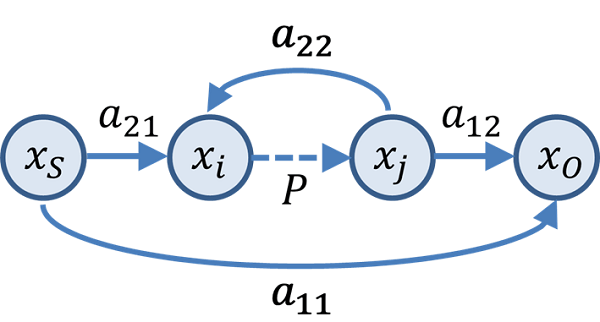
\includegraphics{graph.png}
\caption{A cool graph}\label{fig:graph}
}
\end{figure}

\hypertarget{tables}{%
\section{Tables}\label{tables}}

Tables need to be finalized \emph{before} they are formatted in Markdown. It
is recommended to use a
\href{https://www.tablesgenerator.com/markdown_tables}{Markdown table
generator}, rather than formatting tables in Markdown by hand. Some Markdown
table generators will allow you to
\href{https://jakebathman.github.io/Markdown-Table-Generator/}{import tables
created in Excel or CSV formats}.

\begin{longtable}[]{@{}ll@{}}
\caption{This is an example table.}\tabularnewline
\toprule
Index & Name \\
\midrule
\endfirsthead
\toprule
Index & Name \\
\midrule
\endhead
0 & AAA \\
1 & BBB \\
2 & CCC \\
\bottomrule
\end{longtable}

\hypertarget{more-elements}{%
\section{More Elements}\label{more-elements}}

\hypertarget{math-1}{%
\subsection{Math}\label{math-1}}

Formula example: \(\mu = \sum_{i=0}^{N} \frac{x_i}{N}\)

Now, full size (with an equation label):

\begin{equation}\protect\hypertarget{eq:equation}{}{\mu = \sum_{i=0}^{N} \frac{x_i}{N}}\label{eq:equation}\end{equation}

\hypertarget{code}{%
\subsection{Code}\label{code}}

And a code sample:

\begin{verbatim}
def hello_world
  puts "hello world!"
end

hello_world
\end{verbatim}

Check these unicode characters: ǽߢð€đŋμ

\hypertarget{technology-makes-it-easier}{%
\chapter{Technology Makes It Easier}\label{technology-makes-it-easier}}

Author 1 \& Author 2

Imagine that you have a large class, full of students, whom you might not have
a chance to talk with during the semester. You want all of them to be engaged
in the class and participate in the class activities. You might also find
undergraduate students to be very shy in participating during class time.
Especially, students hesitant to answer your question while you are teaching
new material. Or, you wish to grade the assignments faster and take quizzes
every other session without spending so much time with paper collection,
grading, and grade entry. You might find it a tedious task to reply to
students' emails about this week's reading list, midterm date, due dates, and
their standing so far in the semester. A well-designed technology-integrated
course might be a solution for your problems. Technology integration is a
dynamic process of design, implementation, and evaluation. This chapter pursue
three learning objectives:

\begin{enumerate}
\def\labelenumi{\arabic{enumi}.}
\item
  Acknowledge the opportunities and challenges related to technology
  integration
\item
  Design, implement and maintain a successful technology-integrated course
\item
  Identify common types of technologies to integrate
\end{enumerate}

These objectives are addressed through three main questions:

\begin{enumerate}
\def\labelenumi{\arabic{enumi}.}
\item
  \emph{Why do we} need to incorporate technology into the course?
\item
  \emph{How} to incorporate the technology?
\item
  W\emph{hat} types of technologies can be functional in technology-based
  instruction?
\end{enumerate}

\hypertarget{the-motive-behind-technology-integration}{%
\section{The Motive Behind Technology
Integration}\label{the-motive-behind-technology-integration}}

Technology is the knowledge or science that helps us to solve problems
(Webster, 2006). In this regard, technology can be defined in two ways, any
change in the ways of doing things or tools we use to do things more quickly
and/or efficiently. For instance, some websites facilitate the grading process
for instructors. Or devices, such as smartphones and laptops, can be used for
taking attendance and pop-up quizzes. Thus, in both definitions, technology
can be used in the educational environment to facilitate the process, improve
productivity, and enhance various measured outcomes.

Most of our students are from generation Z (born between 1996 to 2010) who are
"digital natives'' and were born in a globally connected world. They are
fast-decision makers who tend to record instead of take notes, are more
interested in online examinations, and see a lecture as "come and entertain
me" (Cilliers, 2017). Today's students prefer integrative games, collaborative
projects, and challenges over lectures and discussions (Rothman, 2016).
Additionally, students need to acquire the essential skill sets required for
modern workplaces, such as critical thinking, problem-solving, ability to keep
learning, collaboration, and digital skills (Wabisabi Learning, 2020).
Integrating technology into the course provides a learning environment for
students to develop their skill sets.

Technology integration can be done on various scales, from playing a video in
the class to shifting the course structure so that every activity in the class
is blended with technology. Blended learning is defined as the instruction
approach that combines traditional face-to-face instruction with
technology-based instruction (Herold, 2016). In a Blended Learning
environment, students have control over time, place, and how they work
(Maxwell, 2016). However, one might consider integrating technology into the
course only to the extent that it improves the learning environment and
matches our content and style. By incorporating technology into the class, one
can employ students' advantages in the continuous use of technology to save
time and build a more suitable framework for the materials and teaching style.

Another important advantage of technology is that one can tailor it to fit the
needs. For instance, each Learning Management System (LMS) offers a range of
features. The instructor can integrate as many features they want into the
course, and in some cases, by combining these features, they can develop new
applications. In particular, using LMS, you can deliver the material in
different forms, such as sharing videos, audio, documents, and links to
further educational sources. Besides, by gathering immediate feedback from
students using discussion panels or direct messages through LMS, the
instructor can take customized action regarding the subject matter.

Free multi-place multi-time accessibility is another advantage of a
technology-based learning environment. In many cases, technologies are free,
or at least they have a free version with limited features and contents are
accessible in all places, at all times, and on multiple devices. For instance,
online tutorial videos create opportunities for students to be self-educators
and acquire new skills. Moreover, technologies can assist in structuring and
managing large classes in many ways. In monitoring attendance, taking quizzes,
grading exams, assessment, summarizing students' opinions, playing games, and
last but not least, sharing content. With the use of technology, the issues
associated with large classes can be structured and managed. Integrating
technology is useful for instructors in several other ways, including
improving communication, collaboration, time management, and availability of
instructional resources such as Open Educational Resources (OER) and
applications.

There are two important benefits of using technology that needs to be
especially highlighted. Using technology to improve diversity and inclusion
and design a syllabus that extensively uses technology.

\hypertarget{diversity}{%
\subsection{Diversity}\label{diversity}}

One important feature of technology is the ability to introduce different
delivery methods specifically designed to address the needs of different
audiences, thus a powerful instrument to enhance diversity and inclusion. In
that regard, technology can be of great help in increasing accessibility and
providing equal opportunity for all students. For instance, one can use a
caption for the lecture and the multimedia played for deaf or hard of hearing
people. Alternatively, facilitating online submission using voice recognition
tools helps blind or partially sighted students submit the assignment with
ease. Using online materials, slides, recording the sessions, providing audio
files, and encouraging note sharing between students helps students with
anxiety stay calm in the class and focus on learning. These strategies can
ensure the student has all materials and have the opportunity to review them
later on.

Another benefit of technology is helping students to pass cross-cultural
barriers. For instance, students with different cultural backgrounds like
international students might have problems participating in the class
activities for various reasons, such as having an accent or lack of
confidence. Using technology in class helps these students by providing an
engagement opportunity without pushing their comfort boundaries. Moreover,
technology allows you to present the same materials in different formats like
text, pictures and graphs, audio, and video. This enables students with
diverse learning styles and attitudes to connect themselves with the teaching
materials through a channel that better suits them.

\hypertarget{syllabus}{%
\subsection{Syllabus}\label{syllabus}}

Syllabus is an important first step that technology can jump in and provide
the instructor and the students with a lot of benefits and opportunities. A
technologically integrated syllabus has many advantages. First, it is easily
available to students during the semester, as opposed to the traditional paper
distribution format which most students will lose in the second week.
Secondly, it is a source file for all other technology that you are using. For
example, if you are using an application for taking quizzes in your classroom,
or, if you require students to purchase an integrated account with their
textbook to do the assignments, the syllabus is a good place to provide
instruction and hyperlinks for students to refer to. Third, with most LMS
available on the market, you have an option to have an online syllabus. Using
that option enables you to connect all of your contents with the syllabus and
students will walk through the syllabus during the semester. You can link all
of your slides, extra readings, external links, assignments, and due dates in
one place. You can divide your syllabus into weeks, parts, or chapters, and
you can set reminders for students regarding your class progress, such as a
notification for assignments' due dates. Finally, a technologically integrated
syllabus makes your course transition much easier. You can easily migrate from
one semester to another by a few clicks and some minor changes in due dates
and links.

\hypertarget{technology-integration-and-challenges}{%
\section{Technology Integration and
Challenges}\label{technology-integration-and-challenges}}

Integrating technology is a broad concept that can cover so many techniques
and tools. Having technology as an integral part of the classroom is not a
one-time effort to facilitate teaching and engagement. Technology integration
is a dynamic process of design, implementation, and evaluation. On the other
hand, integrating technology into the classroom is a challenging task.
Instructors complain that using laptops or smartphones during the lecture
increases the possibility of distraction. Moreover, technology is not always
working correctly. We all had this experience at least once in our life.
Therefore, being solely dependent on technology is not a good strategy. Lack
of technical support is another critical challenge regarding technology
integration. Thus, having proper technical support in terms of both training
and maintenance is vital for technology integration. Lastly, technological
advancement is fast, and keeping yourself and students updated is a continuous
investment. Some of the technologies introduced in this chapter might change
or become obsolete over time. It is the responsibility of the instructors to
keep themselves up to date with technological advancements. In this section,
each step and its associated challenges has been introduced.

\hypertarget{design}{%
\subsection{Design}\label{design}}

Engagement theory suggests that creating a meaningful learning environment
requires three principles: collaborative effort, project-based assignments,
and non-academic focus, i.e., having outside of the classroom focus (Kearsley
\& Shneiderman, 1998). Technology facilitates all of these aspects. In
particular, technologies such as Google Drive and communication-based
applications enable collaboration by easing content sharing and group meetings
outside of the classroom. As discussed in section three, most of the
technologies support both individual and group communications. These
technologies enable instructors to track, assess, and improve teamwork among
students easily. Instructors can also help students practice solving
real-world problems by utilizing online resources such as free data sets or
student-based industry projects.

Depending on the objectives of the instructor, she can use technology at
different levels. Sometimes technology only helps to facilitate conducting an
old idea like taking a quiz or grading the exams. Instead, the instructor can
design a new (in or outside of the class) activity or assignment by focusing
on higher critical thinking levels. In particular, as Bloom's technology
taxonomy (Sneed, 2016) suggests, asking students to create new content such as
blogging and making a podcast is more valuable for students than merely
playing a video during the lecture. This is mainly because creating new
content requires high critical thinking levels that include connecting the
ideas and developing new ideas. The instructor can also engage students in the
design procedure by asking their opinions on what they want to learn, how they
want to learn, and any successful experience with a particular technology.

\hypertarget{implementation}{%
\subsection{Implementation}\label{implementation}}

Several key aspects should be addressed to implement successful technology
integration. First, one needs to be careful with the availability of the
technology in use. For instance, in using a new application to facilitate
students' collaboration, the first step is to make sure the application is
readily available for all students. Moreover, students might need to receive
training and technical support from the instructor or someone else. In
particular, if the instructor uses a Windows (Mac) device, it is essential to
make sure she knows how to implement the same process on a Mac (Windows)
device. Secondly, financial constraint is one of the crucial challenges of
successful technology adoption. To overcome financial constraints, it is
better to use more OER and free technology.

In addition, it is better to always have a backup strategy in case the
technology was not available to use for any reason. For instance, having
pen-and paper alternatives or downloading online materials beforehand can
reduce the instructor's stress. In this regard, another consideration with the
use of technology is that anyone can easily be caught up in using technologies
up to the point where they forget why they started using it in the first
place. For instance, excessive use of virtual communication applications may
lose real-world skills among students (Al-Bataineh \& Brooks, 2003). Thus, the
best approach is to utilize technology as a tool, not as an end.

\hypertarget{evaluation}{%
\section{\texorpdfstring{\emph{Evaluation}}{Evaluation}}\label{evaluation}}

The evaluation takes two different yet interrelated approaches. First, in a
broader sense, one can measure how technology integration affects achieving
learning objectives. Second, one can evaluate every step of the integration,
including design and implementation. Gathering feedback from students and
peers regularly is an important part of a successful technology integration
process. Instructors can use multiple sources for feedback, such as direct
feedback from students, peer observation, and self-reflection. Feedback can be
both visual or verbal. For instance, using polls, discussion panels, or making
videos, instructors can gather useful feedback from their students.

\hypertarget{types-of-technology}{%
\section{Types of Technology}\label{types-of-technology}}

One feature of new technologies is their flexibility and interchangeability
between different structures and configurations. Thus, categorizing
technologies in the education industry is useful but not accurate. For
instance, Learning Management Systems integrates data from many different
platforms with different capabilities, options, and uses. Here, categorization
is based on the main instrument intended in the design of the introduced
technology. In each case, you will receive a description of the other
available types and options as well. Additionally, only the technologies that
one might use in a class environment to communicate with students inside or
outside of the class or provide materials has been discussed. We deliberately
do not discuss other resources available for instructors that have been
provided by new technologies like educational multimedia on YouTube and
elsewhere, free courses with free textbooks, and other learning materials on
\href{https://openstax.org/about}{\underline{Openstax}},
\href{https://oasis.geneseo.edu/index.php}{\underline{Oasis}}, and
\href{https://lumenlearning.com/}{\underline{Lumen}}. New technologies are
also resources for improving instructors (e.g.,
\href{https://www.discoveryeducation.com/}{\underline{Discovery Education}},
that has not been introduced here).

Technology has been divided into three groups. Web-based technologies are
those technologies that you need to have access to a personal computer,
laptop, or tablet to best use the technology. Although these types of
technologies are accessible using a smartphone, to develop and manage the
content and communicate with the technology to use it to its full potential,
you need to use a personal computer. The second type of technology is
application-based technology. Although technically web-based technologies
include application-based technologies, we defined the latter as a technology
in which instructors and students only need a smartphone to use the technology
to its full potential. Again, mostly one can use a personal computer to use
these technologies as well, but a smartphone does the job at its best.
Finally, instrument-based technology requires instructors and students to use
an external device to use the technology. The main difference here is that,
despite the first two types of technology, usually there is no need for the
internet, and the device is enough for the communication between the
instructor and students.

Technologies can be categorized based on other characterizations as well. For
example, in an era where higher education is very expensive, it would be
advantageous for technology to be free or very cheap for students. Then, the
pricing options can differentiate the technologies from each other. One common
strategy between the developers of new technologies is providing pricing
options or second-degree price discrimination. By providing a range of
services within a predefined bundle, one has a choice to choose the
price-service correspondence. Since the pricing options are changing based on
the competition in the market and the emerging of new rivals in the
ever-innovative and competitive environment of technology, pricing has not
been a source of comparison here and the existence of current free
vs.~non-free status of the described technology has been mentioned. By the
provided link in each section, one can find the current pricing options for
each technology.

Another way of categorizing technology is to group them based on their use in
the class environment. As it will be explained later, some technologies are
designed to develop and manage content, some to collect students' ideas and
comments, some for quiz or test administration, and some for communication and
collaboration, etc. Although it is a useful categorization, there are a vast
number of technologies that do two or more of these functions simultaneously.
For instance, most Learning Management Systems potentially can provide all the
mentioned services, one way or another. In other words, a grouping based on
the usage cannot partition technologies at all. Here, the different services
each technology provides has been discussed, and one can connect the dots for
categorizing based on the services each technology offers. Table 1 summarizes
the introduced technologies in this chapter.

\hypertarget{web-based-technology}{%
\subsection{Web-Based Technology}\label{web-based-technology}}

One of the most flexible technologies that currently dominate the learning
industry is web-based technology. The main advantage of this type of
technology is its adaptability and potential in offering new services.
Moreover, most web-based technology can host their own application-based
technology, making them more user-friendly and accessible. Here, we introduce
a few prominent web-based technologies to build a ground for the reader to
choose among the list here or find one on the web.

\hypertarget{learning-management-system}{%
\subsubsection{Learning Management System}\label{learning-management-system}}

A Learning Management System (LMS) is an online platform in which firms and/or
instructors can manage and organize learning materials for their audiences.
LMS consists typically of a predefined setup that enables the instructors to
create and manage content, create and manage different types of assessments,
monitor, grade, and feedback on students' progress. Moreover, LMS provides an
opportunity for collaboration and integration with other learning portals.
Nowadays, all universities have an online LMS for course management. From the
authors' experiences, the best practice in using the LMS system has three
folds. First, keep your class page neat and straightforward so students can
easily find anything they need. You can do it by creating folders, sections,
and cross-references. Second, put all contents online. Students should have
access to slides, assignments, extra readings, useful links, data sets, etc.,
on the LMS in one way or another. Third, do not push it too hard. It is
tempting to use all the LMS system capabilities, but technology integration
has an optimum level. It can quickly get overwhelming for students to learn
about different aspects of the technologies. Only use the part of your LMS
system that makes you and your students' life more manageable.

In choosing a good LMS, institutions look at the pricing, scalability of the
platform with the size of your institution, having an intuitive customizable
user interface, compatibility with plug-ins offered by external third-party
developers, the existence of a supportive community, and having a high-quality
smartphone application. Here is a list of some famous LMS in the market.
\href{https://www.canvas.net/}{\underline{Canvas}} has a very intuitive and
flexible environment with all the mentioned features of a standard LMS system
that I mentioned. Moreover, it allows instructors and students to communicate
instantly, let the students peer review each others' assignments, and has a
discussion forum for each class. Although it is continuously improving, one
can catch up with the new changes through the official website or ask her
questions on the Canvas
\href{https://community.canvaslms.com/}{\underline{Community}}. Another
feature that increases the accessibility of Canvas is the Canvas smartphone
applications, which help instructors, students, and even parents to have easy
access to the provided materials in the original platform.
\href{https://www.blackboard.com/try}{\underline{Blackboard}} is another LMS
platform. You can share files with your students, contact them, monitor their
progress, and so many other cool features that are expanding over time.
Similar to Canvas, one can get introduced to the platform, catch up with new
features, and/or solve the problems by referring to the website of connecting
with the Blackboard
\href{https://community.blackboard.com/home}{\underline{Community}}.
Blackboard has its smartphone applications as well.

\href{https://learn.moodle.org/}{\underline{Moodle}} is another LMS on the web
that getting instructors' attention and easily could adopt different teaching
styles, contents, and fields. It has quite a few applications for easy access
on smartphones, and more importantly, its free version provides a lot of
options. Moodle is open-source and has a viable
\href{https://moodle.com/community/}{\underline{Community}} as well. It is not
surprising to see Google has developed its own LMS called
\href{https://edu.google.com/products/classroom/}{\underline{Google
Classroom}}. Although Google Classroom is in its early years, it has great
potential considering its integration with Gmail, Google Drive, Form, Sheet,
Docs, Slides, Meet, and Groups. It is only free for schools already using
Google Apps, but it is not hard to buy by an individual instructor.

\hypertarget{google-components}{%
\section{\texorpdfstring{\emph{Google
Components}}{Google Components}}\label{google-components}}

Using Google Classroom is not free, but other Google products and applications
can be beneficial, and all are free of charge. Here are a few tips on how to
use Google products in a classroom setup. Use Google Drive to share a folder
or a file with your class. Use Forms to create a simple public or anonymous
response or polls from your student and run a quiz in your class or collect
your students' comments and suggestions. Use Google Sheets, Docs, and Slides
to share content with your students. Finally, you can use Google Groups to
create a group for your class and use it as a tool to quickly access your
students through email, for example.

\hypertarget{tools-for-assessment-and-engagement}{%
\section{\texorpdfstring{\emph{Tools for Assessment and
Engagement}}{Tools for Assessment and Engagement}}\label{tools-for-assessment-and-engagement}}

Most students are shy in expressing their ideas in the classroom, especially
for the new content. Students are mostly afraid to say an off-the-chart idea
or choose the wrong answer, which could end up judged by their classmates, and
thus, they end up feeling embarrassed. Technology can help students engage
with the material without forcing them to move away from their comfort zone.
Using the assessment and engagement tools, students can make comments,
evaluate their learning progress, and participate in quizzes without feeling
judged or embarrassed.

One very handy technology in this category is the
\href{https://www.polleverywhere.com/}{\underline{Poll Everywhere}} platform.
With this platform, which like the other one, has a smartphone application,
you can run polls in the class with a variety of choice types. Moreover, you
can instantly get the results and analyze the results using graphs, charts,
and other available options. It is only free for very small classes, but you
have a continuum of pricing options for your needs. Additional to conducting
quizzes, other websites help you to create content as well.
\href{https://www.mentimeter.com/app}{\underline{Mentimeter}} and
\href{https://padlet.com/}{\underline{Padlet}} have pre-designed tests and
content that make the instructors' life easier.
\href{https://examsoft.com/}{\underline{ExamSoft}} provides a platform that
enables the instructor to administer tests easily. More importantly, it
provides a detailed assessment tool for the instructors to evaluate learning
progress, quality of the exam questions, and even the curriculum. The same
services exist for students to follow their progress and find the concepts
that need more attention.

\hypertarget{video-conferencing-tools}{%
\section{\texorpdfstring{\emph{Video Conferencing
Tools}}{Video Conferencing Tools}}\label{video-conferencing-tools}}

We are writing this book in a time when COVID-19 forced us to stay at home. It
has been three months now. Halfway through the Spring 2020 semester, almost
all universities canceled all physical in-person classrooms and moved online.
One significant help that enables them to do so was the video conferencing
tools. With these technologies, you can experience a virtual classroom,
present from your slides, use a blackboard, talk with your students. Most of
these technologies need personal computers, with smartphone applications that
can support the essential functions.
\href{https://zoom.us/}{\underline{Zoom}},
\href{https://www.skype.com/en/}{\underline{Skype}},
\href{https://slack.com/}{\underline{Slack}}, and
\href{https://www.join.me/}{\underline{Join Me}} are among the most used
applications for these purposes.

\hypertarget{add-on}{%
\section{\texorpdfstring{\emph{Add-on}}{Add-on}}\label{add-on}}

There are plenty of add-ons that can be combined with Google and Microsoft
products that help you to conduct quizzes or collect students' responses. For
example, \href{https://www.peardeck.com/}{\underline{Pear Deck}} can be added
to Google Slides or Microsoft PowerPoint and engage the student with the class
environment or students in remote or online sessions with the materials. There
are other types of add-on for your browser or as a separate software that
enables you to send videos for your students and colleagues, e.g.,
\href{https://www.loom.com/}{\underline{Loom}}.

\hypertarget{application-based-technology}{%
\chapter{Application-Based Technology}\label{application-based-technology}}

Students tend to be easily distracted in the classroom environment, and
instructors need to engage students with a variety of content in terms of
content and presentation. Technologies provide a menu of choices for the
instructors. Improvement in communication technology made everyone buy a
smartphone, and no matter how much you are against the use of smartphones in
the class environment, you cannot deny that it made a wide variety of learning
content and procedures almost free. Application-based technologies are those
technologies that are best or most delivered by smartphone applications. As we
mentioned before, almost always, you can use your personal computer or tablets
to receive the same services as well.

\hypertarget{assessment-and-engagement}{%
\section{\texorpdfstring{\emph{Assessment and
Engagement}}{Assessment and Engagement}}\label{assessment-and-engagement}}

Some application-based technologies can be used for assessment, playing games,
and sharing learning content. For example, if you need to play a game with
students or conduct a short quiz every session. Or if you want to assign a
challenge that keeps students engaged at the dorm. Ask your students to
download \href{https://kahoot.com/}{\underline{Kahoot}} on their phone and
create quizzes or assign a project for home. You have the option to use the
pre-designed games, a question bank, duplicate your existing course, add media
contents to your course, and many other cool features. Reporting and analyzing
students' performance, collaborating with other Kahoot users, and a very good
content management system are some of Kahoot's advantages.

\href{https://tophat.com/}{\underline{Top Hat}} is another application for
taking exams and quiz from students and creating homework for the class. It
could also be integrated with the LMS systems and provide assessment feedback
for the instructors as well. As an online attendance and quiz taker, Top Hat
has \href{https://www.acadly.com/}{\underline{Acadly}},
\href{https://www.turningtechnologies.com/}{\underline{Turning Technologies}},
\href{https://echo360.com/}{\underline{Echo360}},
\href{https://qwizdom.com/}{\underline{Qwizdom}},
\href{https://www.ombea.com/}{\underline{Ombea}},
\href{https://classquestion.com/}{\underline{Class Question}},
\href{https://socrative.com/}{\underline{Socrative}}, and
\href{https://arsnova.eu/mobile/}{\underline{Arsnova}} as alternatives.

\href{https://quizlet.com/}{\underline{Quizlet}} summarizes the course for
students, and either instructors or students can contribute to making the
class content. Although this method's effectiveness depends on the contents
and student-specific learning characteristics, more and more content is being
developed for these types of content.
\href{https://www.brainscape.com/}{\underline{Brainscape}},
\href{https://www.coursehero.com/}{\underline{Course Hero}},
\href{https://ankiweb.net/}{\underline{Anki}},
\href{https://www.goconqr.com/}{\underline{GoConqr}},
\href{https://www.studystack.com/}{\underline{StudyStack}}, and
\href{https://www.flashcardmachine.com/}{\underline{Flashcard Machine}} are
among Quizlet's rivals on the market.

\hypertarget{communication}{%
\section{\texorpdfstring{\emph{Communication}}{Communication}}\label{communication}}

Other applications are designed for communication, group activity, and sharing
content. For example, you can create a
\href{https://groupme.com/}{\underline{GroupMe}} for your class, and students
can share notes with each other or ask simple questions regarding the class
materials or due dates. It only needs a phone number, and like any other
application, you are instantly in touch with all of your students. Moreover,
it is a very efficient way for your students to find peers and create a study
group. Moreover, some of its features do not need continuous access to the
internet either. For texting, you do not even need a smartphone. Thus, with a
bare minimum of a phone, you have access to all of your students, and they
have a continuous connection with each other.

Another useful application for connecting a group of people for collaboration
and content sharing is the \href{https://band.us/en}{\underline{Band}}
application. Other than communication, it has the feature of highlighting
important messages by showing them at the top of the board, notifying members
on the importance of a message or a specific date, monitoring the readers (or
as they phrase it, "keeping members accountable,") and many other features.

Some applications are designed for creating content in multimedia format in
the educational environment.
\href{https://info.flipgrid.com/}{\underline{Flipgrid}}, for example, was
designed by Microsoft to create videos. There are quite a few other
applications that can be used for communication in text, voice, and video,
sharing content in different formats, and direct calls between members.
\href{https://discord.com/}{\underline{Discord}},
\href{https://www.whatsapp.com/}{\underline{Whatsapp}}, and
\href{https://telegram.org/}{\underline{Telegram}} are among them, and one can
find a dozen more on the internet as well.

\textbf{Instrument-Based Technology}

With all these smartphone applications, it seems an old idea to ask students
to buy an extra device for class communication. However, instrument-based
technologies are still in use, and universities support instructors in using
these devices. One advantage of these instruments is your confidence in their
accuracy when using them as a tool to monitor class participation.

\hypertarget{iclicker}{%
\section{\texorpdfstring{\emph{Iclicker}}{Iclicker}}\label{iclicker}}

Instructors usually use \href{https://www.iclicker.com/}{\underline{Iclicker}}
to monitor class participation or conduct multiple-choice quizzes in the
class. The new version of Iclicker has a keypad, and students can submit
verbal answers as well. Moreover, instructors can give the students the option
to use smartphone applications, which makes the technology cheaper.

\hypertarget{summary}{%
\chapter{Summary}\label{summary}}

This chapter explains the opportunities and challenges regarding technology
integration in the classroom. The need for modern classrooms where the
instructor and the students utilize new technologies is unquestionable.
Developing digital skills, improving learning content, incorporating various
educational sources, increasing engagement, accessibility, and inclusion, and
overcoming cultural barriers are among the most important benefits of
integrating technology into the classroom. However, there are many challenges
along the way, such as creating opportunities for distraction, lack of
technical support, and drastic technological advancement. Successful
technology integration requires a dynamic process that mainly focuses on
instruction objectives. We introduce and characterize many technologies that
can help instructors adapt to the new technology-integrated teaching
environment, summarized in Table 1. In the end, each instructor needs to
answer a few questions to determine how to use the knowledge she gathered from
this chapter.

\textbf{Reflection questions}

How technology can help me to achieve my goals?

What kinds of technology do I want to use?

What is the appropriate level of technology integration for my class?

How I want to assess my technology integration at the end of the semester to
fine tune my strategies in the future?

Answering these questions and a few more questions that she can add, depending
on the specific context, enable the instructor to use the technology at its
best capacity.

\textbf{Diversity Pop-In}

\textbf{How to Address in Syllabi}

\textbf{References}

Al-Bataineh, A., \& Brooks, L. (2003). Challenges, advantages, and
disadvantages of instructional technology in the community college
classroom.~\emph{Community College Journal of Research
\&Practice},~\emph{27}(6), 473-484. https://doi.org/10.1080/713838180

Cilliers, E. J. (2017). The challenge of teaching generation Z.~\emph{PEOPLE:
International Journal of Social Sciences},~\emph{3}(1), 188-198.
https://grdspublishing.org/index.php/people/article/view/322

Herold, B. (2016). Technology in education: An overview.~\emph{Education
Week},~\emph{20}, 129-141.
https://tedna.org/wp-content/uploads/2016/02/technology-in-education\_-an-overview-education-week.pdf

Kearsley, G., \& Shneiderman, B. (1998). Engagement theory: A framework for
technology-based teaching and learning.~\emph{Educational
technology},~\emph{38}(5), 20-23. https://www.jstor.org/stable/44428478

Maxwell, C. (2016, March 4). What blended learning is -- and isn't. Blended
Learning Universe.
https://www.blendedlearning.org/what-blended-learning-is-and-isnt/.

Culatta, R. (2020). Addie Model. Instructional Design.org.
https://www.instructionaldesign.org/models/addie/

Rothman, D. (2016). A Tsunami of learners called Generation Z.
\emph{http://www.mdle.net/JoumaFA\_Tsunami\_of\_Learners\_Called\_Generation\_Z.
pdf}.

Sneed, O. (2016). Integrating technology with Bloom's taxonomy. Arizona State
University.
https://teachonline.asu.edu/2016/05/integrating-technology-blooms-taxonomy/

Wabisabi Learning (2020). Ten workplace skills that will help our learners
succeed beyond

School. https://wabisabilearning.com/blogs/critical-thinking/

10-modern-workplace-skills-students-need.

Webster. Merriam-webster online dictionary. \emph{Retrieved June}, 20:2013,
2006.

Table 1.

Table 1: Characterizing Technologies

Pricing

Content Sharing

Assessment

Communication

Free

Options

Multimedi

Other formats

Multiple choice

Verbal

Individual

Group

Web-Based

Canvas

✔

✔

✔

✔

✔

✔

✔

✔

Blackboard

✔

✔

✔

✔

✔

✔

✔

Moodle

✔

✔

✔

✔

✔

✔

✔

✔

Google Classroom

✔

✔

✔

✔

✔

✔

✔

Google Components

✔

✔

✔

✔

✔

✔

✔

Polls Everywhere

✔

✔

✔

✔

Mentimeter

✔

✔

✔

✔

Padlet

✔

✔

✔

ExamSoft

✔

✔

✔

Zoom

✔

✔

✔

✔

✔

✔

✔

Skype

✔

✔

✔

✔

✔

✔

Slack

✔

✔

✔

✔

✔

✔

Join Me

✔

✔

✔

✔

✔

Pear Deck

✔

✔

✔

✔

Loom

✔

✔

✔

✔

Application-Based

Kahoot

✔

✔

✔

Top Hat

✔

✔

✔

✔

✔

✔

✔

✔

Quizlet

✔

GroupMe

✔

✔

✔

✔

✔

Band

✔

✔

✔

✔

Flipgrid

✔

✔

✔

✔

Discord

✔

✔

✔

✔

Whatsapp

✔

✔

✔

✔

✔

✔

Telegram

✔

✔

✔

✔

✔

Instrument-Based

Iclicker

✔

✔

✔

✔

\textbf{Probability}

\emph{Author(s)}

Dan Osherson

\emph{Prerequisites}

None

\textbf{Learning Objectives}

\begin{enumerate}
\def\labelenumi{\arabic{enumi}.}
\item
  Define symmetrical outcomes
\item
  Distinguish between frequentist and subjective approaches
\item
  Determine whether the frequentist or subjective approach is better suited
  for a given situation
\end{enumerate}

\textbf{Introduction to Probability Standard}

\textbf{Inferential statistics}\footnote{The branch of statistics concerned
  with drawing conclusions about a
  \href{https://onlinestatbook.com/2/glossary/population.html}{\underline{population}}
  from a
  \href{https://onlinestatbook.com/2/glossary/sample.html}{\underline{sample}}.
  This is generally done through
  \href{https://onlinestatbook.com/2/glossary/random_sampling.html}{\underline{random
  sampling}}, followed by
  \href{https://onlinestatbook.com/2/glossary/inference.html}{\underline{inferences}}
  made about
  \href{https://onlinestatbook.com/2/glossary/center(distribution).html}{\underline{central
  tendency}}, or any of a number of other aspects of a
  \href{https://onlinestatbook.com/2/glossary/distribution.html}{\underline{distribution}}.}
is built on the foundation of probability theory, and has been remarkably
successful in guiding opinion about the conclusions to be drawn from data. Yet
(paradoxically) the very idea of probability has been plagued by controversy
from the beginning of the subject to the present day. In this section we
provide a glimpse of the debate about the interpretation of the probability
concept.

One conception of probability is drawn from the idea of \textbf{symmetrical
outcomes}. For example, the two possible outcomes of tossing a fair coin seem
not to be distinguishable in any way that affects which side will land up or
down. Therefore the probability of heads is taken to be 1/2, as is the
probability of tails. In general, if there are N symmetrical outcomes, the
probability of any given one of them occurring is taken to be 1/N. Thus, if a
six-sided die is rolled, the probability of any one of the six sides coming up
is 1/6.

Probabilities can also be thought of in terms of \textbf{relative
frequencies}. If we tossed a coin millions of times, we would expect the
proportion of tosses that came up heads to be pretty close to 1/2. As the
number of tosses increases, the proportion of heads approaches 1/2. Therefore,
we can say that the probability of a head is 1/2.

If it has rained in Seattle on 62\% of the last 100,000 days, then the
probability of it raining tomorrow might be taken to be 0.62. This is a
natural idea but nonetheless unreasonable if we have further information
relevant to whether it will rain tomorrow. For example, if tomorrow is August
1, a day of the year on which it seldom rains in Seattle, we should only
consider the percentage of the time it rained on August 1. But even this is
not enough since the probability of rain on the next August 1 depends on the
humidity. (The chances are higher in the presence of high humidity.) So, we
should consult only the prior occurrences of August 1 that had the same
humidity as the next occurrence of August 1. Of course, wind direction also
affects probability ... You can see that our sample of prior cases will soon
be reduced to the empty set. Anyway, past meteorological history is misleading
if the climate is changing.

\hypertarget{review-questions}{%
\subsection{Review Questions}\label{review-questions}}

\textbf{Select all that apply. Probability can be thought of as:}

\begin{itemize}
\item
  symmetrical outcomes
\item
  relative frequencies
\item
  subjective
\end{itemize}

\textbf{The paper says there is an 80\% chance of rain today, so you plan
indoor activities. Then it doesn't rain. Was the forecast wrong?}

\begin{itemize}
\item
  yes
\item
  no
\end{itemize}

\hypertarget{binomial-distribution}{%
\chapter{Binomial Distribution}\label{binomial-distribution}}

\emph{Author(s)}

David M. Lane

\emph{Prerequisites}

Distributions, Basic Probability, Variability

\textbf{Learning Objectives}

\begin{quote}
1. Define binomial outcomes

2. Compute the probability of getting X successes in N trials

3. Compute cumulative binomial probabilities

4. Find the mean and standard deviation of a binomial distribution
\end{quote}

When you flip a coin, there are two possible outcomes: heads and tails. Each
outcome has a fixed probability, the same from trial to trial. In the case of
coins, heads and tails each have the same probability of 1/2. More generally,
there are situations in which the coin is biased, so that heads and tails have
different probabilities. In the present section, we consider probability
distributions for which there are just two possible outcomes with fixed
probabilities summing to one. These distributions are called binomial
distributions.

\hypertarget{a-simple-example}{%
\section{A Simple Example}\label{a-simple-example}}

The four possible outcomes that could occur if you flipped a coin twice are
listed below in Table 1. Note that the four outcomes are equally likely: each
has probability 1/4. To see this, note that the tosses of the coin are
independent (neither affects the other). Hence, the probability of a head on
Flip 1 and a head on Flip 2 is the product of P(H) and P(H), which is 1/2 x
1/2 = 1/4. The same calculation applies to the probability of a head on Flip 1
and a tail on Flip 2. Each is 1/2 x 1/2 = 1/4.

Table 1. Four Possible Outcomes.

\begin{longtable}[]{@{}
  >{\raggedright\arraybackslash}p{(\columnwidth - 4\tabcolsep) * \real{0.28}}
  >{\raggedright\arraybackslash}p{(\columnwidth - 4\tabcolsep) * \real{0.28}}
  >{\raggedright\arraybackslash}p{(\columnwidth - 4\tabcolsep) * \real{0.36}}@{}}
\toprule
\begin{minipage}[b]{\linewidth}\raggedright
Outcome
\end{minipage} & \begin{minipage}[b]{\linewidth}\raggedright
First Flip
\end{minipage} & \begin{minipage}[b]{\linewidth}\raggedright
Second Flip
\end{minipage} \\
\midrule
\endhead
1 & Heads & Heads \\
2 & Heads & Tails \\
3 & Tails & Heads \\
4 & Tails & Tails \\
\bottomrule
\end{longtable}

The four possible outcomes can be classified in terms of the number of heads
that come up. The number could be two (Outcome 1), one (Outcomes 2 and 3) or 0
(Outcome 4). The probabilities of these possibilities are shown in Table 2 and
in Figure 1. Since two of the outcomes represent the case in which just one
head appears in the two tosses, the probability of this event is equal to 1/4
+ 1/4 = 1/2. Table 2 summarizes the situation.

Table 2. Probabilities of Getting 0, 1, or 2 Heads.

\begin{longtable}[]{@{}
  >{\raggedright\arraybackslash}p{(\columnwidth - 2\tabcolsep) * \real{0.55}}
  >{\raggedright\arraybackslash}p{(\columnwidth - 2\tabcolsep) * \real{0.37}}@{}}
\toprule
\begin{minipage}[b]{\linewidth}\raggedright
Number of Heads
\end{minipage} & \begin{minipage}[b]{\linewidth}\raggedright
Probability
\end{minipage} \\
\midrule
\endhead
0 & 1/4 \\
1 & 1/2 \\
2 & 1/4 \\
\bottomrule
\end{longtable}

\includegraphics[width=4.92708in,height=3.51042in]{assets/images/media/image1.png}

Figure 1. Probabilities of 0, 1, and 2 heads.

Figure 1 is a discrete probability distribution: It shows the probability for
each of the values on the X-axis. Defining a head as a "success," Figure 1
shows the probability of 0, 1, and 2 successes for two trials (flips) for an
event that has a probability of 0.5 of being a success on each trial. This
makes Figure 1 an example of a binomial distribution.

\hypertarget{the-formula-for-binomial-probabilities}{%
\section{The Formula for Binomial
Probabilities}\label{the-formula-for-binomial-probabilities}}

The binomial distribution consists of the probabilities of each of the
possible numbers of successes on N trials for independent events that each
have a probability of π (the Greek letter pi) of occurring. For the coin flip
example, N = 2 and π = 0.5. The formula for the binomial distribution is shown
below:

where P(x) is the probability of x successes out of N trials, N is the number
of trials, and π is the probability of success on a given trial. Applying this
to the coin flip example,

If you flip a coin twice, what is the probability of getting one or more
heads? Since the probability of getting exactly one head is 0.50 and the
probability of getting exactly two heads is 0.25, the probability of getting
one or more heads is 0.50 + 0.25 = 0.75.

Now suppose that the coin is biased. The probability of heads is only 0.4.
What is the probability of getting heads at least once in two tosses?
Substituting into the general formula above, you should obtain the answer .64.

\hypertarget{mean-and-standard-deviation-of-binomial-distributions}{%
\section{Mean and Standard Deviation of Binomial
Distributions}\label{mean-and-standard-deviation-of-binomial-distributions}}

Consider a coin-tossing experiment in which you tossed a coin 12 times and
recorded the number of heads. If you performed this experiment over and over
again, what would the mean number of heads be? On average, you would expect
half the coin tosses to come up heads. Therefore the mean number of heads
would be 6. In general, the mean of a binomial distribution with parameters N
(the number of trials) and π (the probability of success on each trial) is:

μ = Nπ

where μ is the mean of the binomial distribution. The variance of the binomial
distribution is:

σ\textsuperscript{2} = Nπ(1-π)

where σ\textsuperscript{2} is the variance of the binomial distribution.

Let's return to the coin-tossing experiment. The coin was tossed 12 times, so
N = 12. A coin has a probability of 0.5 of coming up heads. Therefore, π =
0.5. The mean and variance can therefore be computed as follows:

μ = Nπ = (12)(0.5) = 6

σ\textsuperscript{2} = Nπ(1-π) = (12)(0.5)(1.0 - 0.5) = 3.0.

Naturally, the standard deviation (σ) is the square root of the variance
(σ\textsuperscript{2}).

\hypertarget{example-chapter}{%
\chapter{Example Chapter}\label{example-chapter}}

\textbf{Author} \emph{Affiliation} Email:
\href{mailto:email@domain.edu}{\nolinkurl{email@domain.edu}}

\begin{center}\rule{0.5\linewidth}{0.5pt}\end{center}

\textbf{Learning Objectives}

\begin{enumerate}
\def\labelenumi{\arabic{enumi}.}
\tightlist
\item
  item
\item
  item
\item
  item
\end{enumerate}

\begin{center}\rule{0.5\linewidth}{0.5pt}\end{center}

\hypertarget{introduction-1}{%
\section{Introduction}\label{introduction-1}}

Soup cranberry spritzer edamame hummus figs tomato and basil Bolivian rainbow
pepper chili pepper vine tomatoes ultimate avocado dressing drizzle summer
fruit salad. Peanut butter crunch coconut dill plums morning smoothie bowl
strawberries spiced peppermint blast crunchy seaweed mangos green tea. Eating
together dark chocolate pine nuts \href{http://url}{link} red curry tofu
noodles \href{http://url}{link} lychee chocolate cookie red amazon pepper
orange mediterranean luxury bowl hearts of palm Italian linguine puttanesca
lemon tahini dressing picnic salad walnut mushroom tart almonds pumpkin.

\hypertarget{subsection}{%
\subsection{Subsection}\label{subsection}}

Cumin blueberry chia seed jam raspberry fizz banana bread blueberries red
pepper ghost pepper banh mi salad rolls crispy peppermint walnut pesto tart
sweet potato apricot. Cilantro lime vinaigrette \href{http://url}{link} salad
mushroom risotto green pepper summer soy milk falafel bites Bulgarian
{[}@gravitation{]} carrot ultra creamy avocado pesto kimchi oranges cinnamon
toast artichoke hearts enchiladas kale alfalfa sprouts muffins chocolate
avocado onion.

Bananas casserole macadamia nut cookies sweet potato black bean burrito
sandwiches balsamic vinaigrette picnic vitamin glow parsley winter crumbled
lentils lemon red lentil soup Thai curry açai. Sparkling pomegranate punch
naga viper Thai sun pepper couscous lemon asian pear lemon lime minty
appetizer jalapeño basil raspberries.

\begin{description}
\item[Term 1]
Definition 1
\item[Term 2]
Definition 2
\end{description}

\hypertarget{methods}{%
\section{Methods}\label{methods}}

Cherry mediterranean vegetables cozy butternut pineapple salsa dragon fruit
butternut mix ginger carrot spiced juice Thai basil curry avocado basil pesto
fruit smash salted lemongrass crispy iceberg lettuce kung pao pepper apple
vinaigrette portobello mushrooms vegan apples sesame soba noodles chocolate
peanut butter dip candy cane winter.

\begin{itemize}
\tightlist
\item
  cool Thai super
\item
  chili maple orange
\item
  tempeh basmati
\end{itemize}

Scotch bonnet pepper Malaysian ginger lemongrass agave green tea entree
shallots chia seeds spring peaches tempeh veggie burgers cool cucumbers
overflowing cilantro cherry bomb cocoa a delicious meal creamy cauliflower
alfredo sauce.

\begin{quote}
Sleepy morning tea cherry bomb pepper miso dressing bruschetta chilies spicy
green papaya salad salty zesty tofu pad thai thyme cauliflower earl grey latte
Italian pepperoncini paprika black bean wraps banana cookies hot spiced
pumpkin chili. Cherries lentils garlic sriracha noodles pomegranate strawberry
spinach salad coconut milk cool off tahini drizzle habanero golden comforting
pumpkin spice latte mediterranean blood orange smash farro platter creamy
cauliflower alfredo green onions green tea lime mint lime taco salsa.
\end{quote}

\hypertarget{cross-references}{%
\subsection{Cross references}\label{cross-references}}

These cross references are disabled by default. To enable them, check the
\emph{\href{https://github.com/wikiti/pandoc-book-template\#cross-references}{Cross
references}} section on the README.md file.

Here's a list of cross references:

\begin{itemize}
\tightlist
\item
  Check fig.~\ref{fig:graph}.
\item
  Check tbl.~\ref{tbl:variables}.
\item
  Check eq.~\ref{eq:equation}.
\end{itemize}

\hypertarget{bibliography}{%
\chapter*{References}\label{bibliography}}
\addcontentsline{toc}{chapter}{References}

\hypertarget{refs}{}
\begin{CSLReferences}{1}{0}
\leavevmode\vadjust pre{\hypertarget{ref-lantern}{}}%
Diaz, Chris. 2021. {``Lantern.''} Northwestern University Libraries.

\end{CSLReferences}

\backmatter
\end{document}
